\section{Turing Machines}
\begin{figure}[h!]	
	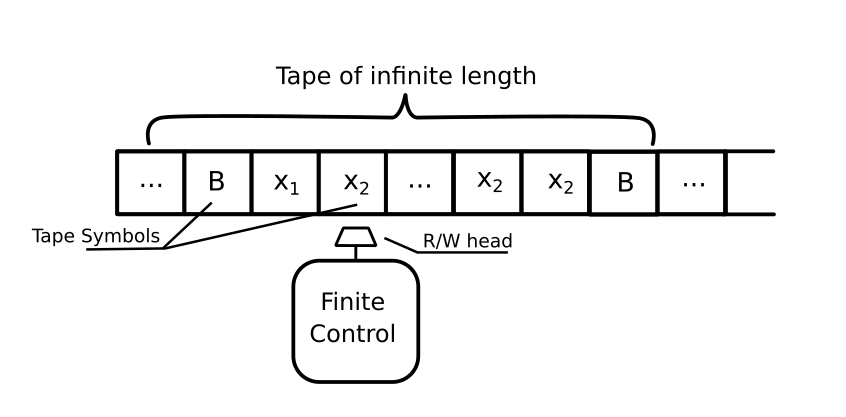
\includegraphics[width=1\textwidth]{images/TuringMachine.png}\par
	\caption{A Turing Machine}
	\label{fig:turingmachine}
\end{figure}

A Turing machine contains four main elements:\\
(a) a program, rather like an ordinary computer which tells what to do for a given instruction;\\ 
(b) a finite state control, which acts like a stripped-down microprocessor, co-ordinating the other operations of the machine; \\
(c) a tape, which acts like a computer memory; and \\
(d) a read- write tape-head, which points to the position on the tape which is currently readable or writable.\\
The finite state control for a Turing machine consists of a finite set of internal states, {$ q_1 , . . . , q_m $}. The number m is allowed to be varied; it turns out that for m sufficiently large this does not affect the power of the machine in any essential way, so without loss of generality we may suppose that m is some fixed constant. Along with these m states, there are two more states, the starting state{$ q_s $} and the halting state {$ q_h $} which denotes the starting and the end of the process respectively. This means that when the processing starts machine will be in the starting state, and when the process is completed, the state control changes to the halting state. These states can be thought of as the internal storage of the machine which helps in the processing.\\
The Turing machine tape is a one-dimensional object, which stretches off to infinity in one direction. The tape consists of an infinite sequence of tape squares numbered 0,1,2,... . The tape squares each contain one symbol drawn from some alphabet, {$ \Gamma $}, which contains a finite number of distinct symbols. The first symbol is always fixed (say {$ \rhd $}) denoting the left edge(starting) of the tape.\\
The tape-head points at a single square in the tape and is used to read the symbol from that location and write new information.\\
A program is a finite set of orders that are to be executed given an internal state and symbol on the tape. So basically, it's a mapping from {$ <q,x> $} to {$ <q',x',s> $} where q and x are the initial internal state and tape square symbol and q' and x' are the final states and symbol. s defines the movement of the tape-head i.e. after updating the state and symbol where the head should go. It can be 0(stay on the same location), 1(move right) or -1(move left except if on the leftmost square). The commands are generally written as {$ <q,x,q',x',s>$} were symbols means the same as before. So, a command of {$ <q_1,1,q_2,2,1> $}will mean that if we encounter the symbol 1 when the internal state is {$q_1$}, change the state to {$q_2$} and overwrite the symbol to 2. Then move the cursor one square towards the right.\\
A lot of modifications are possible in the turing machines. For e.g.: There may be two tapes instead of one in the machine. These modifications may simplify the algorithm used but they don't offer much computational advantage and can actually be shown to be equivalent to the normal turing machines. Hence, we consider only the simple turing machine as described above.

\subsection{Universal Turing Machine}
In a given turing machine, we can vary the program, the internal states and the contents of the tape. But it turns out that we can use a single machine called the {\it Universal Turing Machine} in place of the all the turing machines.\\
A universal turing machine has a fixed internal state and program. So, the only thing that can vary is the content of the tape. In universal turing machine, we first "tell" the machine which machine it must act as and then the input. These all things, the turing machine details and input for that machine, is given through the tape. The turing machine is specified using the Turing number. A Turing number is a unique number associated with each turing machine.\\
This is very much similar to a programmable computer. All the commands are already stored in the memory and the user has to just tell which program to execute and the inputs for that program. The idea of the universal turing machine allows us to thing of a real machine which can compute any given function (computable by algorithm) \\

\subsection{Church Turing Thesis}
It turns out that this simple model can be used to compute any function which has a definite algorithm. It is stated officially as the{ \it Church-Turing Thesis} :\\
\\{\scshape Church Turing Thesis: } The class of functions computable by a Turing machine corresponds exactly to the class of functions which we would naturally regard as being computable by an algorithm.\\
\\This theorem is very important as it defines what all functions can be computed by a classical computer and by quantum computers too!! Though it is not yet clear that what it means to say "computable by algorithm" and hence there may exist another computational method which may compute a function not computable by turing machines.\\
If we allow randomness too in the model, we get a probabilistic Turing Machine. And hence we get the { \it Strong Church-Turing Thesis} :\\
\\{\scshape Strong Church Turing Thesis: } Any model of computation can be simulated on a probabilistic Turing machine with at most a polynomial increase in the number of elementary operations required.\\
The meaning of polynomial increase is defined in the computational complexity section later.
\subsection{Halting Problem}
This problem is a modification of the Hilbert {\it entscheidungsproblem} which asks whether it is possible to compute all the problems in mathematics. The halting problem is\\\\{\scshape Halting Problem: } Does the machine with Turing number x halt upon input of the number y\\
\\This can easily be seen that the halting problem is equivalent to the Hilbert {\it entscheidungsproblem}.\\
Turing proved that it is not possible on a sub-case where the input is same as turing number and hence answered the Hilbert {\it entscheidungsproblem} with a negation. To show this, he defined a halting function:\\
	\begin{equation}
	h(x) = 
	\begin{cases}
	0 & \text{if machine number x does not halt upon input of x}\\
	1 & \text{if machine number x halts upon input of x}\\
	\end{cases}
	\end{equation}	
If there is an algorithm to solve the halting problem, then there is one to compute h(x). We will show that an algorithm to compute h(x) can't exist. Consider the turing machine running the following pseudo-code:\\\\
\indent \indent \large y = h(x) \\
\indent \indent \large if y=0\\
\indent \indent \indent \indent then halt \\
\indent \indent \large else\\
\indent \indent \indent \indent loop forever \\
\normalsize
\\Clearly the algorithm is completely defined and hence it is possible to make the turing machine. But, if we give this turing machine its own number, we can easily see that we arrive at a contradiction. Hence, h(x) can't be calculated and so, the answer to {\it entscheidungsproblem} is a clear {\bf NO}.

\newpage


